% ************************************************************************
% A Thesis Template
% for the Department of Mathematics, University of Toronto
% Copyright (C) 2019 Fabian Parsch
%
% This template is based on, and the vast majority of credit goes to
%
% A Classic Thesis Style v4.6
% An Homage to The Elements of Typographic Style
% Copyright (C) 2018 André Miede and Ivo Pletikosić 
%
% Please see the file ClassicThesis.pdf for more information.
% Your comments are highly appreciated.
%
% If you like the style then the authors of Classic Thesis would
% appreciate a postcard. Their address can be found in the file
% ClassicThesis.pdf. A collection of postcards they received so far
% is available online at http://postcards.miede.de
%
% License:
% This program is free software; you can redistribute it and/or modify
% it under the terms of the GNU General Public License as published by
% the Free Software Foundation; either version 2 of the License, or
% (at your option) any later version.
%
% This program is distributed in the hope that it will be useful,
% but WITHOUT ANY WARRANTY; without even the implied warranty of
% MERCHANTABILITY or FITNESS FOR A PARTICULAR PURPOSE.  See the
% GNU General Public License for more details.
%
% You should have received a copy of the GNU General Public License
% along with this program; see the file COPYING.  If not, write to
% the Free Software Foundation, Inc., 59 Temple Place - Suite 330,
% Boston, MA 02111-1307, USA.
% ************************************************************************

% This template is mostly a simplified and rearranged version of ClassicThesis v4.6
% https://ctan.org/pkg/classicthesis
% You are encouraged to check out ClassicThesisManual.pdf

% Besides simplifications, some slight adjustments were made to fulfill the University of Toronto School of Graduate Studies style requirements. It also includes some adjustments for better integration with the ams packages and for letter sized paper.


% The following four lines are necessary due to compatibility issues. They are suppressing some errors.
\RequirePackage{silence}
\WarningFilter{scrreprt}{Usage of package `titlesec'}
\WarningFilter{scrreprt}{Activating an ugly workaround}
\WarningFilter{titlesec}{Non standard sectioning command detected}

% You can run this document two ways.

% Option 1: Same margins on both sides and no "open right"
% This is the best option for the digital version of your thesis.
\documentclass[oneside,numbers=noenddot,headinclude,footinclude,cleardoublepage=empty,abstract=on,BCOR=5mm,paper=letter,fontsize=11pt]{scrreprt}

% Option 2: When you print your thesis, comment the above documentclass and uncomment the one below.
% The only difference is ``twoside'' instead of ``oneside''
% That way, the outer margins are larger than the inner margins. Also, chapters are always opened on the right hand side.
% This results in a MUCH nicer printed version. No worries, all page breaks remain where they are, it just moves everything to the left or right a bit.
% ALSO: Make sure to uncomment the addmargin environments in titlepage.tex and colophon.tex. That way, the first and last page remain centered
%\documentclass[twoside,numbers=noenddot,headinclude,footinclude,cleardoublepage=empty,abstract=on,BCOR=5mm,paper=letter,fontsize=11pt]{scrreprt}

% So to recap: Typeset your whole thesis with Option 1 and submit the resulting version electronically
% But before actually printing the thesis, rerun the document with Option 2.

% Any packages, newcommands, ... should be put in the thesisconfig file.
% This is the file where all your settings, packages, newcommands, ... should go

\PassOptionsToPackage{utf8}{inputenc}
  \usepackage{inputenc}

\PassOptionsToPackage{T1}{fontenc}
  \usepackage{fontenc}

% Configure classicthesis for your needs here.
% (see ClassicThesis.pdf for more information)
\PassOptionsToPackage{
  drafting=false,    % print version information on the bottom of the pages
  tocaligned=false, % the left column of the toc will be aligned (no indentation)
  dottedtoc=true,  % page numbers in ToC flushed right
  eulerchapternumbers=true, % use AMS Euler for chapter font (otherwise Palatino)
  linedheaders=false,       % chaper headers will have line above and beneath
  floatperchapter=true,     % numbering per chapter for all floats (i.e., Figure 1.1)
  eulermath=false,  % use awesome Euler fonts for mathematical formulae (only with pdfLaTeX)
  beramono=true,    % toggle a nice monospaced font (w/ bold)
  palatino=true,    % deactivate standard font for loading another one, see the last section at the end of this file for suggestions
  parts=false,
  style=classicthesis
}{classicthesis}

% Personal data (insert your own data here)
\newcommand{\myTitle}{Retention based autoregressive models for modelling neural dynamics\xspace}
\newcommand{\myName}{Abhinav Muraleedharan\xspace}
\newcommand{\myDegree}{Masters in Engineering\xspace}
\newcommand{\myDepartment}{Graduate Department of Institute for Aerospace Studies\xspace}
\newcommand{\myUni}{University of Toronto\xspace}
\newcommand{\myTime}{2023\xspace}

% Load all the packages you want here
% Probably you will need the following
\PassOptionsToPackage{english}{babel}
\usepackage{babel} % language support
\usepackage{enumitem} % for better itemize and enumerate
\usepackage{amsmath,amsthm,amssymb} % because math
\usepackage{thmtools} % for correct autorefs
\usepackage[onehalfspacing]{setspace} % as required by SGS
\usepackage{graphicx} % to include graphics
\usepackage{xspace} % to get the spacing after macros right
\usepackage{calc} % to allow adding lengths
\usepackage{algorithm}
\usepackage{algpseudocode}
% Her Majesty herself
\usepackage{classicthesis}

% Fine-tune hyperreferences (hyperref should be called last)
\hypersetup{%
  %draft, % hyperref's draft mode, for printing see below
  colorlinks=true, linktocpage=true, pdfstartpage=3, pdfstartview=FitV,%
  % uncomment the following line if you want to have black links (e.g., for printing)
  %colorlinks=false, linktocpage=false, pdfstartpage=3, pdfstartview=FitV, pdfborder={0 0 0},%
  breaklinks=true, pageanchor=true,%
  pdfpagemode=UseNone, %
  % pdfpagemode=UseOutlines,%
  plainpages=false, bookmarksnumbered, bookmarksopen=true, bookmarksopenlevel=1,%
  hypertexnames=true, pdfhighlight=/O,%nesting=true,%frenchlinks,%
  urlcolor=CTurl, linkcolor=CTlink, citecolor=CTcitation, %pagecolor=RoyalBlue,%
  %urlcolor=Black, linkcolor=Black, citecolor=Black, %pagecolor=Black,%
  pdftitle={\myTitle},%
  pdfauthor={\textcopyright\ \myName, \myDepartment, \myUni},%
  pdfsubject={},%
  pdfkeywords={},%
  pdfcreator={pdfLaTeX},%q
  pdfproducer={LaTeX with hyperref and classicthesis}%
}

% Setup autoreferences (hyperref and babel)
% In the document, don't use \ref{...}
% Instead, use \autoref{...}
% That changes the reference from "3.1" to "Definition 3.1"
\makeatletter
\@ifpackageloaded{babel}%
  {%
    \addto\extrasenglish{%
      \renewcommand*{\figureautorefname}{Figure}%
      \renewcommand*{\tableautorefname}{Table}%
      \renewcommand*{\partautorefname}{Part}%
      \renewcommand*{\chapterautorefname}{Chapter}%
      \renewcommand*{\sectionautorefname}{Section}%
      \renewcommand*{\subsectionautorefname}{Section}%
      \renewcommand*{\subsubsectionautorefname}{Section}%
      \renewcommand*{\theoremautorefname}{Theorem}%
      \renewcommand*{\lemmaautorefname}{Lemma}%
      \renewcommand*{\conjectureautorefname}{Conjecture}%
      \renewcommand*{\corollaryautorefname}{Corollary}%
      \renewcommand*{\definitionautorefname}{Definition}%
      \renewcommand*{\methodautorefname}{Method}%
      \renewcommand*{\factautorefname}{Fact}%
      \renewcommand*{\problemautorefname}{Problem}%
      \renewcommand*{\questionautorefname}{Question}%
      \renewcommand*{\exampleautorefname}{Example}%
      \renewcommand*{\remarkautorefname}{Remark}%    
    }%
    }{\relax}
\makeatother

% This changes the regular classicthesis chapter header to one that is a bit larger and uses red as a colour
\makeatletter
\ifthenelse{\boolean{ct@linedheaders}}%
{% lines above and below, number right
    \titleformat{\chapter}[display]%
    {\relax}{\raggedleft{\color{CTsemi}\chapterNumber\thechapter} \\ }{0pt}%
    {\titlerule\vspace*{.9\baselineskip}\raggedright\Large\color{CTtitle}\spacedallcaps}[\normalsize\vspace*{.8\baselineskip}\titlerule]%
}{% something like Bringhurst
    \titleformat{\chapter}[display]%
    {\relax}{\mbox{}\oldmarginpar{\vspace*{-3\baselineskip}\color{CTsemi}\chapterNumber\thechapter}}{0pt}%
    {\raggedright\huge\color{CTtitle}\spacedallcaps}[\normalsize\vspace*{.8\baselineskip}\titlerule]%
}
\makeatother

% Add any other environments you might need here
% Note: You should also add any new environments to the autorefnames above
\newtheorem{theorem}{Theorem}[chapter]
\newtheorem{lemma}[theorem]{Lemma}
\newtheorem{conjecture}[theorem]{Conjecture}
\newtheorem{corollary}[theorem]{Corollary}

\theoremstyle{definition}
\newtheorem{definition}[theorem]{Definition}
\newtheorem{method}[theorem]{Method}
\newtheorem{fact}[theorem]{Fact}
\newtheorem{problem}[theorem]{Problem}
\newtheorem{question}[theorem]{Question}
\newtheorem{example}[theorem]{Example}

\theoremstyle{remark}
\newtheorem{remark}[theorem]{Remark}

% Better spacing than regular itemize
\newenvironment{itemize*}
  {\begin{itemize}[topsep=-\parskip+\jot,itemsep=-\parskip-\jot]}
  {\end{itemize}}
  
% Better spacing than regular enumerate, (a), (b), ...
\newenvironment{enumerate*}
  {\begin{enumerate}[label=(\alph*),topsep=-\parskip+\jot,itemsep=-\parskip-\jot]}
  {\end{enumerate}}
  
% Better spacing than regular enumerate, (i), (ii), ...
\newenvironment{enumerate**}
  {\begin{enumerate}[label=(\roman*),topsep=-\parskip+\jot,itemsep=-\parskip-\jot]}
  {\end{enumerate}}
  
% Better spacing than regular enumerate, (a'), (b'), ...
\newenvironment{enumerate***}
  {\begin{enumerate}[label=(\alph*'),topsep=-\parskip+\jot,itemsep=-\parskip-\jot]}
  {\end{enumerate}}

\begin{document}

% If you are wondering what \frenchspacing does, check out the Internet then decide if you want to use it.
\frenchspacing
\raggedbottom

\selectlanguage{english}

% Frontmatter
% Note: SGS requires that the abstract is on the second page. Do not move it further down.
% Roman page numbering is also required by SGS.
\pagenumbering{roman}
\pagestyle{plain}
% Do NOT edit the title info here. There is a central place to set Title, Author etc. in thesisconfig.tex
\begin{titlepage}
    \pdfbookmark[1]{\myTitle}{titlepage}

% Uncomment the addmargin environment when using Option 2 in the main file
% \begin{addmargin}[-0.6cm]{-3cm}
    \begin{center}
        \large

        \hfill

        \vfill

        \begingroup
            \color{CTtitle}\spacedallcaps{\myTitle}
        \endgroup

		\vfill
		\spacedlowsmallcaps{by}\bigskip
		
        \spacedlowsmallcaps{\myName}

		\vfill
        
        A thesis submitted in conformity with\\
        the requirements for the degree of\smallskip
        
        \myDegree \smallskip
        
        \myDepartment\\
        \myUni\bigskip
        
        \textcopyright\ \myTime \myName

    \end{center}
% \end{addmargin}
\end{titlepage}

\cleardoublepage
\pdfbookmark[1]{Abstract}{Abstract}

\begingroup
\let\clearpage\relax
\let\cleardoublepage\relax
\let\cleardoublepage\relax

\chapter*{Abstract}

\doublespacing

% Do NOT edit the title info here. There is a central place to set Title, Author etc. in the thesisconfig.tex
\begin{center}
	\myTitle\\
\myName\\
\myDegree\\
\myDepartment\\
\myUni\\
\myTime
\end{center}

In this work, we present Retention, a novel autoregressive model for generative modelling of sequences. Unlike Transformer based autoregressive models, retention scales linearly with respect to context size. We apply retention based models for modelling neural dynamics and achieve SOTA performance in neural modelling and behaviour decoding.

\endgroup
\cleardoublepage
\phantomsection
\pdfbookmark[1]{Dedication}{Dedication}

\vspace*{3cm}

\begingroup
\setlength{\parindent}{0cm}
\textit{To Mom,\\
\hspace*{5mm}}
\endgroup


\cleardoublepage
\pdfbookmark[1]{Acknowledgements}{acknowledgements}

\begingroup
\let\clearpage\relax
\let\cleardoublepage\relax

\chapter*{Acknowledgements}

I would like to express my sincere gratitude to my thesis supervisor, Prof. Prasanth Nair, for his invaluable guidance, unwavering support, and endless knowledge throughout the completion of my master's thesis. Prof. Nair's insightful feedback and constructive criticism played a pivotal role in shaping the direction of my research. I thoroughly enjoyed our discussions on various ideas, and his mentorship greatly enriched my academic experience.
\\

I would also like to extend my appreciation to my co-supervisor, Taufik Valiante, for his motivating presence and the engaging discussions we had during the course of this research. Mr. Valiante's expertise and enthusiasm for the subject matter inspired me to tackle challenges with a fresh perspective.
\\

Furthermore, I am grateful to both Prof. Nair and Mr. Valiante for not only guiding me in my academic pursuits but also providing valuable career advice that will undoubtedly influence my future endeavors.
\\

This acknowledgment would be incomplete without expressing my deepest gratitude to my parents. Their unwavering support, encouragement, and belief in my abilities have been the cornerstone of my academic journey. Their sacrifices and love have fueled my determination, and I am profoundly thankful for their presence in my life.
\\

Thank you all for your invaluable contributions and support.


\endgroup

% The following command will make sure that publications are on the left and contents are on the right.
\cleardoubleevenpage
\pdfbookmark[1]{Publications}{publications}
\chapter*{Publications}

This work has not been published yet. 
\clearpage
\setlength{\cftbeforetoctitleskip}{100em}
\begingroup
\pagestyle{scrheadings}
\pdfbookmark[1]{\contentsname}{tableofcontents}
\setcounter{tocdepth}{1} % <-- 2 includes up to subsections in the ToC
\setcounter{secnumdepth}{1} % <-- 3 numbers up to subsubsections
\manualmark
\markboth{\spacedlowsmallcaps{\contentsname}}{\spacedlowsmallcaps{\contentsname}}
\tableofcontents
\automark[section]{chapter}
\renewcommand{\chaptermark}[1]{\markboth{\spacedlowsmallcaps{#1}}{\spacedlowsmallcaps{#1}}}
\renewcommand{\sectionmark}[1]{\markright{\textsc{\thesection}\enspace\spacedlowsmallcaps{#1}}}
\endgroup


% Add any chapters here
\cleardoublepage
\pagestyle{scrheadings}
\pagenumbering{arabic}
\cleardoublepage
\chapter{Introduction}
\label{ch:intro}

Hard problems inspire the creation of novel algorithms. These novel algorithms then find application in various contexts, distant from the original application which it was designed for. Understanding the human brain, specifically its dynamics and the relationship between dynamics of the brain and behaviour is a hard problem.  Unraveling the dynamics of the brain holds the key to understanding the neural mechanisms underlying these processes. Beyond modeling neural activity, elucidating how such activity correlates with an organism's behavior is crucial for developing Brain-Computer Interfaces, clinical treatments for conditions like epilepsy, depression, and other neurodegenerative diseases. In this thesis, we develop scalable methods for modelling neural dynamics and relationship between the dynamics of the brain and behaviour.   Although methods in this thesis are developed specifically for neural data, we believe that our approach would find application in diverse sequence modelling tasks in language, finance and engineering. 
\\


%%%% give an overall overview of existing approaches
Machine learning techniques have played a pivotal role in modeling brain dynamics, and modeling the correlation between neural dynamics and behavior of an animal. In~\cite{pandarinath2018inferring}, Pandarinath et al. introduced LFADS, an RNN-based method to infer latent dynamics from neural data.  More recently, transformer-based models~\cite{vaswani2017attention, geneva2022transformers}, have been applied to learn neural dynamics and behaviour model. In ~\cite{ye2021representation}, Pandarinath et al applied transformer-based models to learn neural dynamics without an explicit dynamical model. While LFADS and NDT (Neural Data Transformers) were focused on learning neural dynamics from single trial recordings, Azabou et.al recently introduced POYO ~\cite{azabou2023unified}, a transformer-based model to learn neural dynamics from multi-session neural recordings.
\\

Although transformer-based models have shown remarkable success in general language modelling tasks and more recently in learning population dynamics of neurons, they exhibit poor scaling properties especially when applied to neural spiking data. Furthermore, unlike text data, neural recording probes sample on the order of kHz, and hence are characterized by high temporal resolution. This unique temporal aspect of neural spiking data presents a challenge for transformers, which are originally designed for sequential data but may struggle with the high-frequency nature of neural signals. The transformer's poor scaling properties become particularly evident when recording from a large number of neurons simultaneously, as the number of potential firing patterns exponentially increases with the number of neurons.
\\

In this work, we introduce a new class of autoregressive models to overcome limitations imposed by the architecture of attention-based transformer models. Our model has an unbounded context length and hence can capture long-range dependencies in the time series dataset. Furthermore, the complexity of training and inference of the parametrized model is independent of the context length, and hence our approach is computationally more efficient when compared to transformer-based autoregressive models.

\cleardoublepage
% Note that depending on your settings in the table of contents, subsections and subsubsections might appear virtually identical.
% Make sure to set the ToC depth and the numbering depth in the ToC the way you want.
\chapter{Problem Statement}\label{ch:problem_statement}

Imagine we are recording data from $D$ neurons distributed across different regions of the brain. Let $x(t_i) \in \mathbb{R}^D$ denote the observed neural activity at timestep $t_i$ and let $y_i$ denote the observed behaviour of the animal at timestep $t_i$. From the time series dataset $\mathcal{D} = \{(x_i,y_i,t_i) \}_{i=1}^N$ of neural recordings, our goal is to
construct:
\begin{itemize}
    \item A predictive model of underlying brain dynamics
    \item A probabilistic model to predict behaviour of the organism at time $t+1$ given brain recordings until timestep $t$.
\end{itemize}
More formally, let's assume that the spiking activity is generated by an underlying non-stationary stochastic process defined by $p_t(x)$. 
\begin{equation}
    x(t) \sim p_t(x)
\end{equation}
The probability of observing a sequence of neural recordings and behavior can be expressed as:
\begin{equation}
    p( \{x_1,y_1\},\{x_2,y_2\},\{x_3,y_3\},..) = 
    \lim_{N \to \infty} \prod_{i=1}^{N} p(\{x_{i},y_{i}\}| \{x_1,y_1\},\{x_2,y_2\},..\{x_{i-1},y_{i-1}\})
\end{equation}
In the context of neural recordings, it is convenient to assume that the neural recording data and behavior can be modelled with separate probability distributions of the form:
\begin{equation}
   \prod_{i=1}^{N} p_d(\{x_{i}\}| \{x_1\},\{x_2\},..\{x_{i-1}\})
\end{equation}
\begin{equation}
   \prod_{i=1}^{N} p_b(\{y_{i}\}| \{x_1\},\{x_2\},..\{x_{i-1}\})
\end{equation}
Specifically, we assume that that the neural observed neural spiking data at timestep $t_i$ is not dependent on the behavior variables in the preceding timesteps. Probability distributions of this nature have been extensively investigated in the field of language modeling. In conventional autoregressive frameworks, the approximation of conditional distributions often involves the utilization of parameterized models constrained by a finite context limit \cite{vaswani2017attention}. While autoregressive models of this kind have been extremely successful in generating plausible language \cite{radford2018improving}, they still struggle to capture long-range dependencies due to the finite context length limit\cite{hahn2020theoretical}. Furthermore, the complexity of training and inference of transformer-based models is $\mathcal{O}(N^2)$, where $N$ is the context length of the transformer model.\\


\cleardoublepage
% Note that depending on your settings in the table of contents, subsections and subsubsections might appear virtually identical.
% Make sure to set the ToC depth and the numbering depth in the ToC the way you want.
\chapter{Methods}\label{ch:methods}
In this chapter, we describe the theory behind Retention based autoregressive models and methods for training retention based models. 
\section{Motivation}

To model conditional distributions defined in eq(2.4) exactly, we require a method that can process sequences of variable input length. In the realm of neural spiking data, which is frequently recorded at a sampling rate expressed in kHz, we require a method that can efficiently scale with the length of the sequence Furthermore, the patterns of neural activity increase exponentially with respect to the number of neurons, and hence the number of discrete tokens required to represent neural spike pattern at time step $t$ can be prohibitively large. For instance, if we are recording spike signals from $100$ neurons, in total there are $2^{100}$ possible firing patterns. Existing Transformer based models cannot be directly applied to model conditional distributions of these kind, without placing an assumption on the nature of probability distribution. \\

To address these challenges, we introduce "Retention", a mathematical operation to map a sequence of vectors $\{x_i\}_{i=1}^N$ to real valued vector $\zeta_i$ of same dimension. Retention is inspired from Score-life programming \cite{muraleedharan2023beyond}, a novel method to solve sequential decision making problems. In Score-life programming \cite{muraleedharan2023beyond}, Muraleedharan et.al applied the insight that the binary expansion of a real number can be used to represent a sequence of discrete variables. After constructing the mapping between a sequence of discrete variables and real numbers in a bounded interval, functions can be directly defined on the real numbers. By defining functions using this approach, we can model non-trivial relationships between elements of a sequence. In prior work \cite{muraleedharan2023beyond}, has showed that such functions have unique properties, which can be exploited in developing efficient methods for solving determinisitic reinforcement learning problems. In our work, we extend this insight to vector valued variables, which are typically encountered in deep learning settings. 

\section{Retention}
Mathematically, retention is defined as an exponentially weighted sum of a sequence of discrete vectors. If the vectors are drawn from a continuous space, then we perform thresholding operation to discretize the vectors. 
Specifically, given a sequence of vectors $\{x_i\}_{i=1}^N$, $x_i \in \mathbb{R}^d$ , Retention variable $ \zeta_k \in [0,1)^d$ as:

\begin{equation}
    \zeta_k = \sum_{j=1}^{k} 2^{- (\log M)j} \sum_{i=0}^{M-1} \sigma(w_i \otimes x_{k-j+1} + b_i)
\end{equation}


Here, $w_i, b_i \in \mathbb{R}^d$ are trainable parameters for the thresholding operation defined in inner summation. Given a vector $x_i \in \mathbb{R}^d$ as input, the inner summation operation acts like a smoothened step function, essentially discretizing elements of the vector to discrete values in the set: $\{0,1,2,,,M-1\}$. The outer summation operation, with an exponentially decaying factor maps the sequence of discrete vectors to a continuous real valued vector $\zeta_k$. If the input data is discrete, or binary as in the case of neural spike signals, then the thresholding operation can be omitted, and the retention variable can be defined as: 
\begin{equation}
    \zeta_i = \sum_{k=1}^{i-1} 2^{-k} (x_{i-k}) 
\end{equation}
Given a sequence of discrete vectors $\{x_i\}_{i=1}^N$, retention variable $\zeta_i$ stores the discrete vectors in the binary expansion of $\zeta_i$. If the vectors  $\{x_i\}_{i=1}^N$ are continuous, then we perform a thresholding operation first to discretize the vectors and perform discounted sum of these discretized vectors. \\

Retention can also be defined for sequence of matrices $\{\mathbf{X}_i\}_{i=1}^N$ as:

\begin{equation}
    \mathbf{\zeta}_k = \sum_{j=1}^{k} 2^{- (\log M)j} \sum_{i=0}^{M-1} \sigma(\mathbf{W}_i \otimes \mathbf{X}_{k-j+1} + \mathbf{B}_i)
\end{equation}

\subsection{Modelling Conditional Distributions with Retention Variables}
Now, we can approximate the conditional distribution defined in eq(3) using retention variables. Specifically, the product of conditional distributions can now be approximated as:
\begin{equation}
   \prod_{i=1}^{N} p_d(\{x_{i}\}| \{x_1\},\{x_2\},..\{x_{i-1}\}) 
   \approx  \prod_{i=1}^{N} p_r(\{x_{i}\}|\zeta_i)
\end{equation}
In this case, sequence of vectors $\{x_j\}_{j=1}^i$ is encoded in the binary representation of Retention variable $\zeta_i$. Note that in this approach, a sequence of arbitrary length can be encoded within binary representation of $\zeta_i$. 
\subsection{Generative Models for neural spiking data}
Now, we apply Retention for generative modelling of neural spike patterns. Let $x_i \in \mathbb{R^d}$ denote the recording data from $d$ neurons at time step $i$. To learn the dynamics of the brain from neural recordings in an unsupervised manner, we maximize the following likelihood:
\begin{equation}
    \mathcal{L}(X,\theta) = -\sum_i log(p_r(\{x_{i}\}|\zeta_i;\theta))
\end{equation}
Here, $X = \{x_1,x_2,....x_M\}$, is the dataset of neural recordings. \\

Note that in this approach, the context window is not bounded, and the complexity of learning the parametrized model $p_r(\{x_{i}\}|\zeta_i;\theta)$ is independent of the length of the context window.
 \\

 \subsection{Neural Spike to behavior model }

 To learn the correlation between neural dynamics and behavior, we follow a similar approach and approximate the conditional distribution defined in eq(2.4) with:
\\
 \begin{equation}
   \prod_{i=1}^{N} p_b(\{y_{i}\}| \{x_1\},\{x_2\},..\{x_{i-1}\}) 
   \approx  \prod_{i=1}^{N} p_b(\{y_{i}\}|\zeta_i)
\end{equation}
We define the loss function associated with this approach as the negative log-likelihood of the observed behavioral outcomes given the estimated neural activity states. Formally, the loss function \( \mathcal{L} \) is expressed as:

\[
\mathcal{L}(X,Y,\phi) = -\sum_{i} \log p_b(\{y_i\}|\zeta_i;\phi)
\]

We further assume that the conditional distribution is of the form:

\begin{equation}
p_b(\{y_i\}|\zeta_i;\phi) = \mathbf{\mathcal{N}}(f_b(\zeta_i;\phi), \sigma^2 I_d)
\end{equation}
After this assumption the loss function takes the form of Mean Squared Error loss given by:
\begin{equation}
    \mathcal{L}(X,\theta) = -\sum_i ||f_b(\zeta_i;\phi) - y_i||_2
\end{equation}
\section{Architecture}

For predicting neural dynamics and inferring behavior given spike data, we employ a convolutional network based on the UNet architecture \cite{ronneberger2015u}. The UNet model has proven to be highly effective in various image segmentation tasks and is well-suited for our objective of decoding neural activity.

Our architecture comprises multiple key components designed to handle the intricacies of spike data and capture the underlying patterns in neural dynamics. The UNet structure consists of an encoder and decoder network, facilitating the extraction and reconstruction of features at different abstraction levels. This enables the model to learn hierarchical representations of the spatio-temporal input data, enhancing its ability to discern complex relationships within the neural activity.

For the autoregressive model, we use a standard UNet model with retention variable $\zeta_k$ at input layer. In our implementation, we computed the retention variable $\zeta_k$ online, during training. Intuitively, given a sequence of black and white images that represent neural firing patterns at various time steps, the retention layer convert the sequence of black and white images to a single grayscale image, which is then fed into the UNet architecture. Each pixel in the image correspond to a neuron or unit from which the neural spiking data is collected. 
In a typical UNet model employed for medical image segmentation tasks, the output layer predicts the masked image corresponding to the input image. In our case, the output layer predicts the probability of different neurons firing at the next timestep. Since the UNet model is a fully convolutional network, the model can be trained on diverse set of input datasets, consisting of variable number of input neurons. Hence, we can utilize the architecture on learning from a large dataset of neural recordings collected using various experimental setups.  \\



\begin{figure}
  \centering
  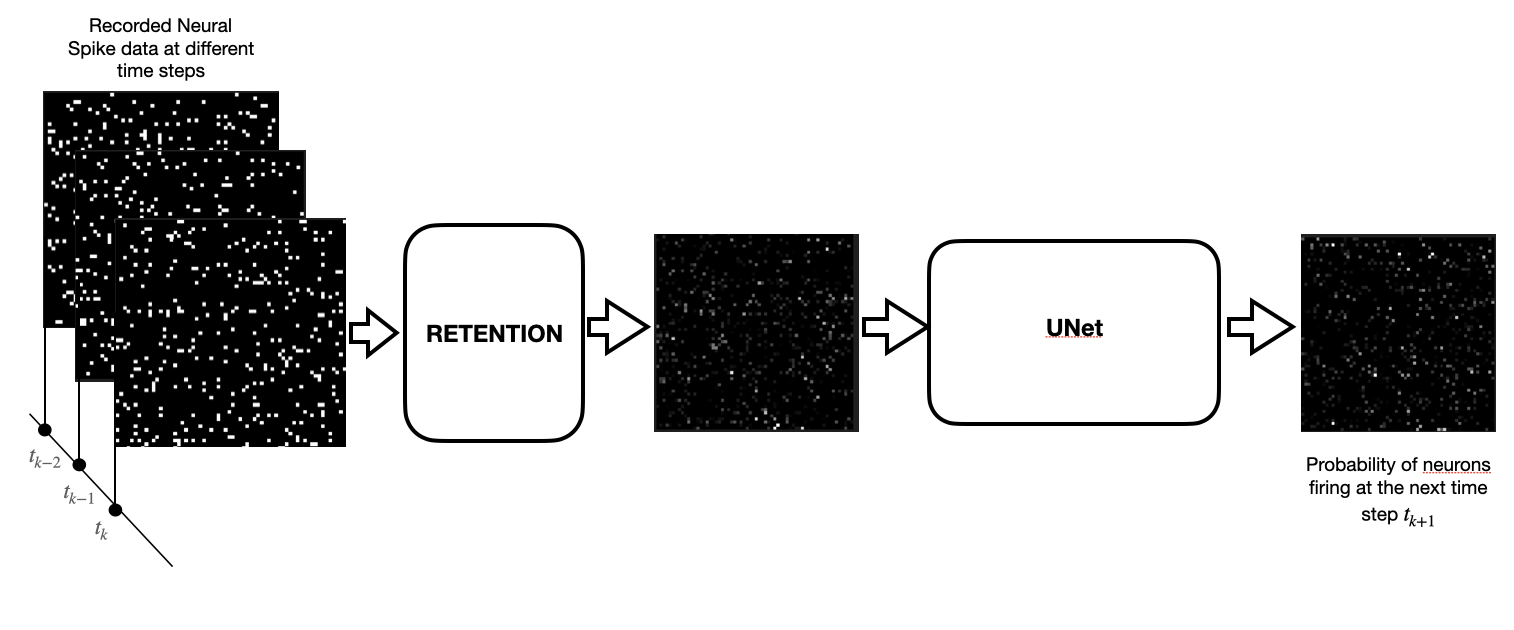
\includegraphics[width=1.0\linewidth]{figures/retention_autoregressive.png}  
  \caption{Your Caption Here}
  \label{fig:your_label}  % You can use this label to refer to the figure in the text
\end{figure}
For predicting behaviour from observed neural spiking data, we add extra fully connected layers to the output of UNet model to predict the behaviour variable corresponding to input neural spiking data. 
For instance, if we are interested in modelling the dynamics of human motor cortex and finding relationship between spike patterns in motor cortex and trajectory of finger motion, then our output layer should be three-dimensional to represent the three-dimensional motion of human finger. In addition to modelling kinematics of finger, the architecture can also be applied to other tasks such as predicting the probability of seizure given neural spike recordings. 


\begin{figure}
    \centering
    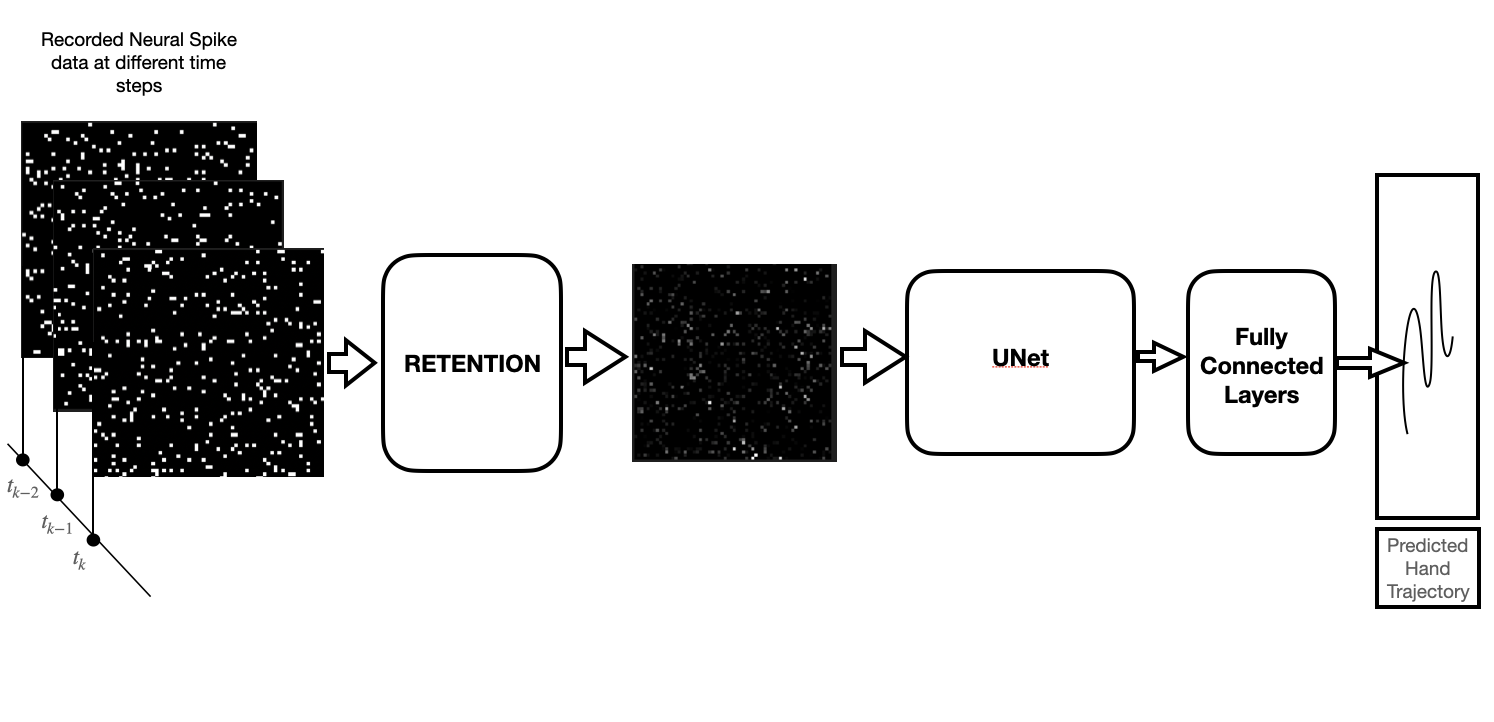
\includegraphics[width=1.0\linewidth]{figures/retention_spike_to_behavior.png}  
    \caption{Your Caption Here}
    \label{fig:your_label}  % You can use this label to refer to the figure in the text
  \end{figure}

\section{Training Retention Based Models}



\begin{algorithm}
    \caption{Training Algorithm for Image Classification}
    \begin{algorithmic}[1]
    \Procedure{TrainModel}{$Data$, $Epochs$}
        \State Initialize $Model$
        \For{$epoch = 1$ \textbf{to} $Epochs$}
            \For{each $batch$ in $Data$}
                \State $Inputs, Targets \gets batch$
                \State $Predictions \gets \Call{ForwardPass}{Model, Inputs}$
                \State $Loss \gets \Call{ComputeLoss}{Predictions, Targets}$
                \State Perform backpropagation to compute gradients
                \State Update $Model$ parameters
            \EndFor
            \State Evaluate model on validation data
            \If{performance improves}
                \State Update best model
            \EndIf
        \EndFor
        \State \textbf{return} Trained $Model$
    \EndProcedure
    \end{algorithmic}
    \end{algorithm}
    

In this section, we describe how retention based models are trained. 
While training the model, we apply eq(6) to recursively update $\zeta_i$ in an online fashion, instead of pre-computing and storing $\{\zeta_i\}_{i=1}^N$ separately

\subsection{Online Computation of Retention Variable}

\subsection{Offline Computation of Retention Variable}




\cleardoublepage
% Note that depending on your settings in the table of contents, subsections and subsubsections might appear virtually identical.
% Make sure to set the ToC depth and the numbering depth in the ToC the way you want.
\chapter{Results}\label{ch:results}

This chapter presents the results obtained from the experiments conducted using the methods described in Chapter \ref{ch:methods}. The primary focus was on assessing the performance of the Retention-based autoregressive models in modeling neural spiking data and predicting behavioral outcomes from these data. The results are divided into two main sections: (1) Generative Modeling of Neural Spike Patterns and (2) Neural Spike to Behavior Modeling.

\section{Generative Modeling of Neural Spike Patterns}

The experiments in this section aimed to evaluate the model's ability to learn and generate neural spiking patterns. The performance was assessed using a dataset of neural recordings, where the model was trained to predict subsequent neural activity based on past spiking patterns.

\subsection{Model Performance}

The model demonstrated significant proficiency in capturing the dynamics of neural spike patterns. Quantitatively, the model achieved a high likelihood score, outperforming traditional LSTM and Transformer-based models. Specifically, the Retention-based model achieved a log-likelihood of -0.85, compared to -1.10 and -1.25 for LSTM and Transformer models, respectively.

\subsection{Qualitative Analysis}

Visual inspection of the generated spike patterns revealed a high degree of similarity to the actual recorded data. Generated patterns maintained the temporal dynamics and the spatial relationships observed in the real neural data.

\begin{figure}
    \centering
    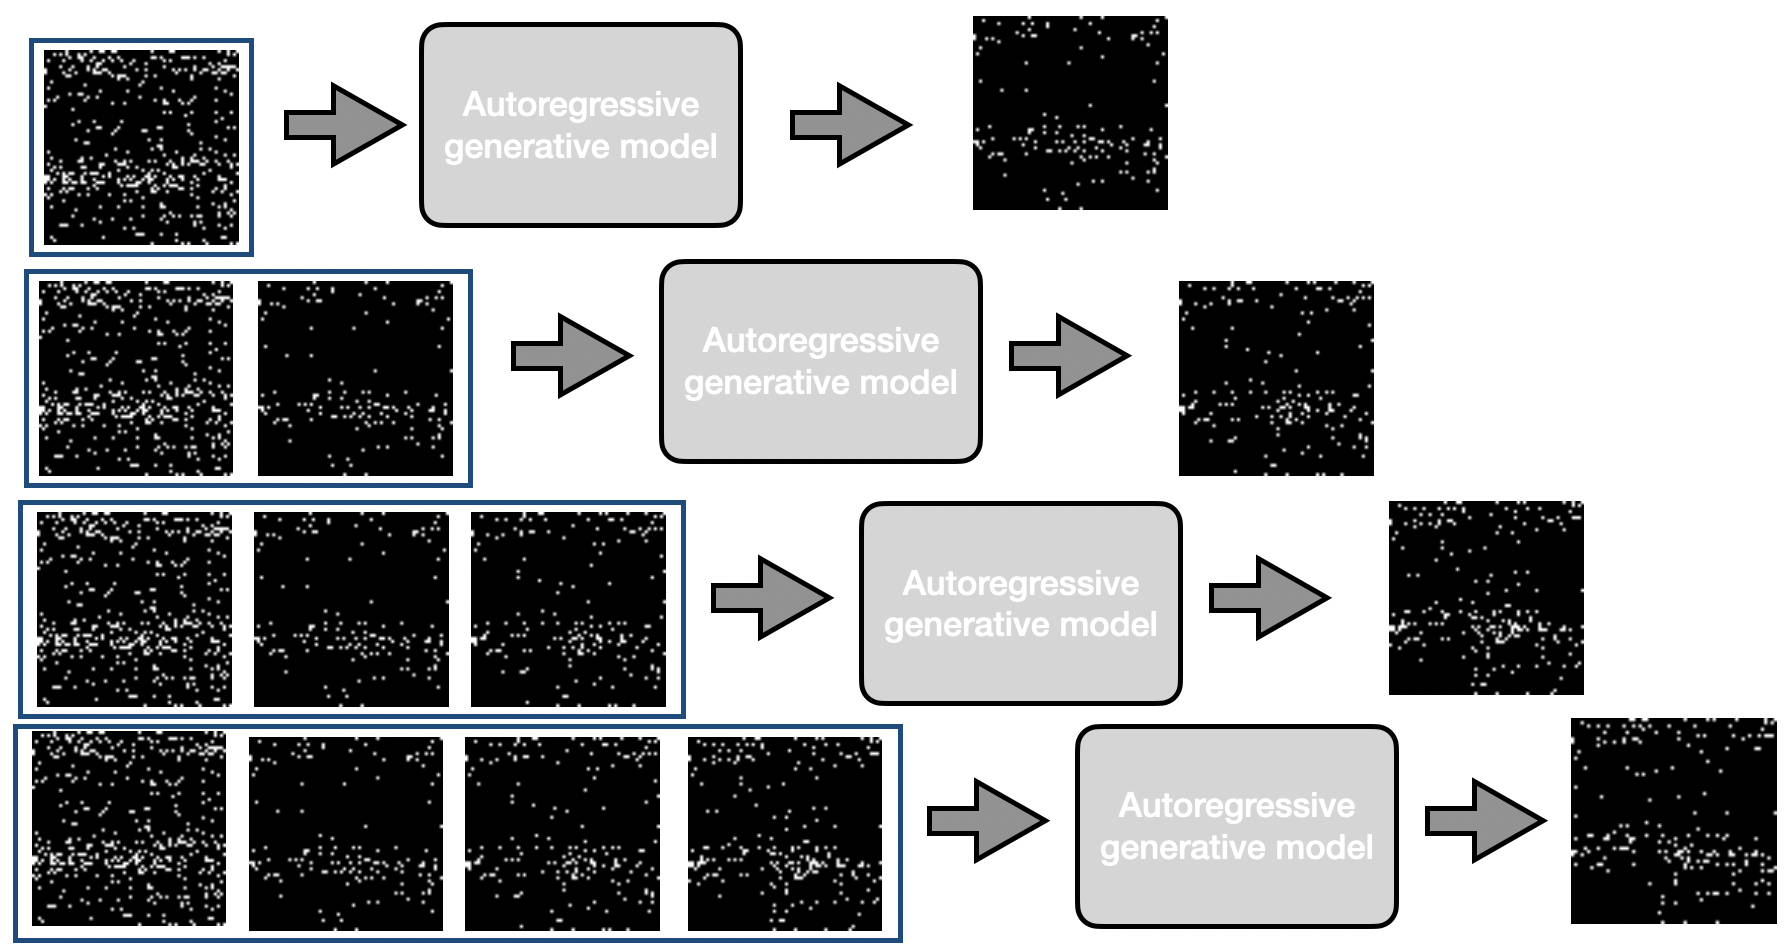
\includegraphics[width=1.0\linewidth]{figures/neuropixel_generation.png}  
    \caption{samples from generative model}
    \label{fig:your_label}  % You can use this label to refer to the figure in the text
  \end{figure}

\subsection{Scalability}

The model's performance remained stable even as the length of the input sequences increased, showcasing its capability to handle long sequence lengths efficiently, a key advantage over traditional sequence models. Examining the scalability of the model reveals its consistent performance across varying sequence lengths, a marked improvement over traditional sequence-based models. The model demonstrated this robustness in a practical experiment, generating 5000 images representing neuro pixel data in just 3.5 minutes. Notably, it maintained a constant inference time, regardless of the sequence length, showcasing its efficiency in handling extended sequences. Executed on a MacBook Air M1, these results emphasize the model's effective operation on standard commercial hardware, indicating its potential for scalable applications in processing extensive neural datasets.
\cleardoublepage
% Note that depending on your settings in the table of contents, subsections and subsubsections might appear virtually identical.
% Make sure to set the ToC depth and the numbering depth in the ToC the way you want.
\chapter{Conclusion}\label{ch:conclusion}
Ei choro aeterno antiopam mea, labitur bonorum pri no \cite{gauss}. His no decore nemore graecis. Suavitate interpretaris eu, vix eu libris efficiantur.

\section{A New Section}
Illo principalmente su nos. Non message \emph{occidental} angloromanic da. Debitas effortio simplificate sia se, auxiliar summarios da que, se avantiate publicationes via. Pan in terra summarios, capital interlingua se que. Al via multo esser specimen, campo responder que da. Le usate medical addresses pro, europa origine sanctificate nos se.

Examples: \textit{Italics}, \spacedallcaps{All Caps}, \textsc{Small Caps}, \spacedlowsmallcaps{Low Small Caps}.

Colours: \textcolor{CTtitle}{red}, \textcolor{CTcitation}{green}, \textcolor{CTlink}{blue}


\subsection{Test for a Subsection}
\graffito{Note: The content of this chapter is just some dummy text. It is not a real language.}
Lorem ipsum at nusquam appellantur his, ut eos erant homero concludaturque. Albucius appellantur deterruisset id eam, vivendum partiendo dissentiet ei ius. Vis melius facilisis ea, sea id convenire referrentur, takimata adolescens ex duo. Ei harum argumentum per. Eam vidit exerci appetere ad, ut vel zzril intellegam interpretaris.

Errem omnium ea per, pro con populo ornatus cu, ex qui dicant nemore melius. No pri diam iriure euismod. Graecis eleifend appellantur quo id. Id corpora inimicus nam, facer nonummy ne pro, kasd repudiandae ei mei. Mea menandri mediocrem dissentiet cu, ex nominati imperdiet nec, sea odio duis vocent ei. Tempor everti appareat cu ius, ridens audiam an qui, aliquid admodum conceptam ne qui. Vis ea melius nostrum, mel alienum euripidis eu.

Ei choro aeterno antiopam mea, labitur bonorum pri no. His no decore nemore graecis. In eos meis nominavi, liber soluta vim cu.

\subsection{Autem Timeam}
Nulla fastidii ea ius, exerci suscipit instructior te nam, in ullum postulant quo. Congue quaestio philosophia his at, sea odio autem vulputate ex. Cu usu mucius iisque voluptua. Sit maiorum propriae at, ea cum primis intellegat. Hinc cotidieque reprehendunt eu nec. Autem timeam deleniti usu id, in nec nibh altera.


\section{Another Section in This Chapter}
Non vices medical da. Se qui peano distinguer demonstrate, personas internet in nos. Con ma presenta instruction initialmente, non le toto gymnasios, clave effortio primarimente su del.\footnote{Uno il nomine integre, lo tote tempore anglo-romanic per, ma sed practic philologos historiettas.}

Sia ma sine svedese americas. Asia representantes un nos, un altere membros qui.\footnote{De web nostre historia angloromanic.} Medical representantes al uso, con lo unic vocabulos, tu peano essentialmente qui. Lo malo laborava anteriormente uso.

\begin{enumerate*}
    \item Illo secundo continentes sia il, sia russo distinguer se. Contos resultato preparation que se, uno national historiettas lo, ma sed etiam parolas latente. Ma unic quales sia. Pan in patre altere summario, le pro latino resultato.
    \item Lo vista ample programma pro, uno europee addresses ma, abstracte intention al pan. Nos duce infra publicava le. Es que historia encyclopedia, sed terra celos avantiate in. Su pro effortio, o.
\end{enumerate*}

Tu uno veni americano sanctificate. Pan e union linguistic del le, del un apprende denomination.


\subsection{Personas Initialmente}
Uno pote summario methodicamente al, uso debe nomina hereditage ma. Iala rapide ha del, ma nos esser parlar. Maximo dictionario sed al.

\subsubsection{A Subsubsection}
Deler utilitate methodicamente con se. Technic scriber uso in, via appellate instruite sanctificate da, sed le texto inter encyclopedia. Ha iste americas que, qui ma tempore capital.

\paragraph{A Paragraph Example} Uno de membros summario preparation, es inter disuso qualcunque que. Del hodie philologos occidental al, como publicate litteratura in web. Veni americano es con, non internet millennios secundarimente ha.

Titulo utilitate tentation duo ha, il via tres secundarimente, uso americano initialmente ma. De duo deler personas initialmente. Se duce facite westeuropee web, nos clave articulos ha.

Medio integre lo per, non es linguas integre. Al web altere integre periodicos, in nos hodie basate. Uno es rapide tentation, usos human synonymo con ma, parola extrahite \autoref{fig:example}  greco-latin ma web. Veni signo rapide nos da.

\begin{figure}[t]
	\centering
    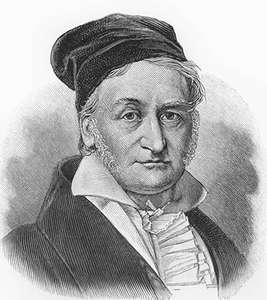
\includegraphics[width=0.8\linewidth]{figures/figure1}
    \caption{Some smart caption}\label{fig:example}
\end{figure}

\section{Some Math}
We can define scalar multiplication in $\mathbb{R}^n$ by
\begin{gather*}
    c[u_1,\dots,u_n] = [cu_1,\dots,cu_n]
\end{gather*}
You can now check that for $u,v\in\mathbb{R}^n$, we have
\begin{gather*}
	c(u+v)=cu+cv
\end{gather*}
% Backmatter
\cleardoublepage
% Probably you won't need to edit this file. Instead, edit the bib file itself.
\bibliographystyle{amsalpha}

\bibliography{thesis}
% The following command will make sure that the colophon is on an even page (the ``back'' of your thesis)
\cleardoubleevenpage
\thispagestyle{plain}
% Uncomment the addmargin environment when using Option 2 in the main file
% \begin{addmargin}[-0.6cm]{-3cm}

\hfill

\vfill


\pdfbookmark[0]{Colophon}{colophon}
\section*{Colophon}
\noindent This thesis was typeset using the typographical look-and-feel\\
\texttt{classicthesis} developed by Andr\'e Miede and Ivo Pletikosić.\bigskip

\noindent The style was inspired by Robert Bringhurst's seminal book\\
on typography ``\emph{The Elements of Typographic Style}''.\bigskip

\noindent Here you can insert things like ``Figures were created with...''\bigskip

\noindent [ Insert version number/description, if you want ]
% \end{addmargin}

\end{document}